%%%%%%%%%%%%%%%%%%%%%%%%%%%%%%%%%%%%%%%%%%
 %Copyright (C) 2018-2020 YuZJ.
%使用CC-BY-NC-SA授权。一份完整版本的许可证已位于附录。这个版本原始作者YuZJ,
%邮箱theafamily@126.com(最后连接于2019年06月20日17:32:17)。
%%%%%%%%%%%%%%%%%%%%%%%%%%%%%%%%%%%%%%%%%%
\part{开始之前}
\chapter{版权}
版权所有\copyright{} 2018-2019 YuZJ Lab. \par
使用CC-BY-NC-SA授权。一份完整版本的许可证已位于附录。这个版本原始作者YuZJ,邮箱\url{theafamily@126.com}(最后连接于2019年06月20日17:32:17)。\par
本书使用了Adobe公司提供的相关字体。包括:
\begin{verbatim}
SourceHanSansSC-Bold.otf
SourceHanSansSC-Regular.otf
SourceHanSerifSC-Bold.otf
SourceHanSerifSC-Regular.otf
\end{verbatim}
字体对应的许可证已经附于附录。
\begin{center}
{\large \bf\color{red}对本文档所引起的任何后果不作担保!}
\end{center}
\chapter{第一版序}
《天工开物·序言》描述当时人们在生产方面的创造时写道:“天覆地载,物号数万,而事亦因之,曲成而不遗。”人类在计算机技术上的创造亦是如此。很高兴生活在信息技术快速发展的新时代,国内外优秀的软件都可以被获取以为我们所用。然而“工欲善其事,必先利其器”,对于我们来说,掌握如何高效率地使用计算机是十分重要的。如一位数学教师可用\LaTeX\footnote{\LaTeX 是一个产生于 \TeX 的一个排版系统。它能够高效地编辑公式,并且能够胜任巨型文档排版和诸如交叉引用、创建索引、管理参考文献资料等复杂的排版任务。注意\LaTeX 不是一个所见即所得的软件。}而不是MS Office \footnote{MS是Microsoft(微软)的缩写,MS Office 是微软公司发布的非自由付费办公套件。} 编辑公式或使用Git\footnote{强大的分布式版本控制系统。官方网站\url{https://git-scm.com/}(最后连接于2019年7月6日21:06:04)。}进行版本控制以高效地管理自己的论文。因此,为了方便信息化教学的开展,我结合自己的工作经历,不自量力“年来著书一种”,为希望掌握关于如何高效地使用教室计算机的初级和高级技巧的电教委员或者其余希望提高计算机技能的教师、学生及其他教职人员编写了这份文件。\par
手册中题为“入门”的章节是针对初学者的,它大致介绍了Windows操作系统和MS Office等软件来实现日常教学,Windows操作系统的简单技巧与最基础的Windows安全。题为“进阶”的章节是针对已有一定技能基础并希望尝试更加有效的Windows安全工具(如使用以GNU/Linux\footnote{对于“GNU/Linux”操作系统的称法一直存在争议。本书为了保持通用性,在参考【Richard Stallman之GNU/Linux问答】\url{https://www.gnu.org/gnu/gnu-linux-faq.html}(最后连接于2019年06月20日17:32:59)的基础上决定使用“GNU/Linux”。关于GNU/Linux的详细介绍参见\pageref{sec:gnulinux}页\ref{sec:gnulinux}。}为操作系统的反病毒光盘清除计算机病毒)的电教委员的。题为“高级”的章简单地节介绍了GNU/Linux 操作系统的入门知识及其教学实现。\par
在介绍多种多样的软件时,我遵循的原则是法律——性能——易用性——价格。在性能相同的情况下,易用性优先。但我也不会忘了推荐一些不错的自由免费软件以减少希望廉价使用正版软件者的开支。\par
在使用这份手册时,最重要的是实践。本人才疏学浅,文本中或许有(大量)错误,请广大读者不吝赐教。联系方式:\url{theafamily@126.com}(最后连接于2019年06月20日17:32:17)。如果文档中存在任何侵权之处,请按邮箱联系。一经确认,将立刻改正。希望在选考中取得优良成绩的“大业文人”,应将本书“弃置案头”。“此书于功名进取,毫不相关也。”\par
时己亥年肆月廿七日,西历2019年5月1日\par
慈溪YuZJ于家之书房
\chapter{第二版序}
在第二版中,我回顾了先前的版本,对于其中的口语等不合适用语进行改进。在学习更多计算机知识后,我深刻地体会到了自己对于核心概念理解程度过浅以及贫乏的语言对于表达的障碍。我将继续改进这一版本,并恳请各位提出意见批评指正。
\chapter{警告}
\begin{enumerate}
\item 本书内所有网络链接在“最后连接时间”前均有效且已经过Norton Safe Web的Edge插件、Microsoft SmartScreen筛选器及卡巴斯基网络反病毒(包含于卡巴斯基免费版2020,病毒库更新时间为检测当天12:00)以及Avira Free Antivirus检测。 
\item 注意,本书中提到的所有应用程序都应该从其官方网站或镜像源处下载。从任何非官方软件发布处(如腾讯电脑管家“软件中心”)下载任何本书中提到的软件是不被推荐的。\par 
\item 从任何网站下载“破解版”或“注册机”“算号器(KeyGen)”“KMS注册机(仅指非法的KMS服务器)”都是不被允许的。这些程序可能含有“后门”或直接携带病毒(主要表现为网络蠕虫(Worm)、特洛伊木马(Trojan)和提权程序(Rootkit))\cite{HR1}\cite{HR2}\cite{HR3}\cite{HR4}\cite{HR5}。\par
如果你确信你的下载站提供了可靠的软件,你需要使用哈希校验来确保文件可靠性。方法:使用7Zip在文件资源管理器中的右键菜单“CRC SHA”选项校验哈希值并于官方提供的哈希值作比较。如果一致,那么这个软件可视为是官方的。
\item 请在安装任何软件时查看最终用户许可声明(EULA)和隐私协议。
\end{enumerate}
经检测的镜像站列表如下(检测于2019年6月22日17:16:47):
\begin{enumerate}
	\item 【清华大学开源软件镜像站 | Tsinghua Open Source Mirro】r\url{https://mirrors.tuna.tsinghua.edu.cn/}
	\item 【USTC Open Source Software Mirror】\url{http://mirrors.ustc.edu.cn/}
	\item 【欢迎访问网易开源镜像站】\url{http://ubuntu.cn99.com/}\url{http://mirrors.163.com/}
	\item 【华为开源镜像站\_软件开发服务\_华为云】\url{https://mirrors.huaweicloud.com/}
	\item 【阿里巴巴开源镜像站】\url{https://opsx.alibaba.com/mirror}
	\item 【兰州大学开源社区镜像站】\url{http://mirror.lzu.edu.cn/}
	\item 【重庆大学开源软件镜像站 | Chongqing University Open Source Mirror Site】 \url{https://mirrors.cqu.edu.cn/}
	\item 【Nanjing University Open Source Mirror Site】\url{https://mirrors.nju.edu.cn/}
	\item 【南京邮电大学开源软件镜像站 | Njupt Open Source Mirror】\url{https://mirrors.njupt.edu.cn/}
	\item 【Mirrors@NWAFU】\url{https://mirrors.nwafu.edu.cn/}
	\item 【】\url{https://mirrors.sohu.com/}
	\item 【SourceForge - Download, Develop and Publish Free Open Source Software】\url{https://sourceforge.net/}
	\item 【FOSSHUB】\url{https://www.fosshub.com/}
	\item 【The world’s leading software development platform · GitHub】\url{https://github.com/}
\end{enumerate}
任何由于违反以上原则导致的问题将不被回复。
\chapter{自由软件、开源软件和专有软件}
我们以是否公开源代码为标准来区分一个软件是不是专有软件。不公开源代码的软件称为“专有软件”(参见\pageref{sec:exe}页的\ref{sec:exe}),而公开源代码的软件称为开源或者自由软件。安装时,正规软件会展示许可证(如下图为安装Filezilla时展示的GNU GPL许可证),你应该仔细地阅读它并决定是否安装。
\begin{center}
	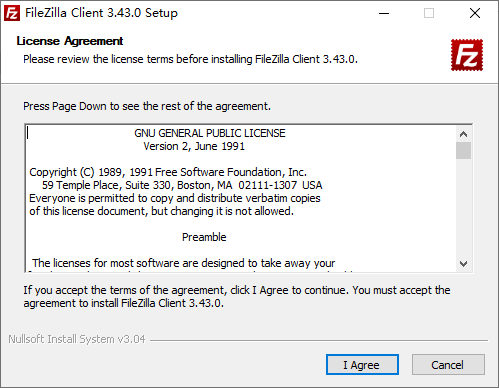
\includegraphics[scale=0.5]{pic/fzi}
\end{center}\par
源代码允许用户“自由”使用的软件称为自由软件。然而,因为“自由”是一个很难定义的名词,因此我们使用Richard Stallman的标准界定“自由”。请参见【Various Licenses and Comments about Them - GNU Project - Free Software Foundation】\url{http://www.gnu.org/licenses/license-list.html}(最后连接于2019年07月30日18:08:02)来确定你的许可证是否自由。\par
我虽然支持自由软件,但是承认拥有\textbf{合法版权}的专有软件的合法性。在这本书中,在\textbf{不影响使用}的前提下如果能完成此功能的专有软件能被自由/开源软件替代,将使用后者。
以下是一些常见问题的解答。
\section{使用自由/开源软件有什么好处?}
价格。无论是专有软件还是自由软件的创造者都有权利因自己的创造得到物质上与精神上的回报,但对于消费者来说,自由软件大多数是免费的,但功能强大的专有软件大部分收费。\par
安全性。(除了研究病毒程序的自由社区以外)自由/开源软件既然敢于将代码和开发过程(指源代码的版本控制机制,任何对源代码的修改一经保存都可以被查到)示人,就说明他们有勇气接受全世界软件开发者和用户的监督。专有软件的代码不开放性决定了恶意代码或“后门”能被非常方便地置入代码中。除此之外,一小部分专有软件会收集大大超过需求的个人信息。\par
维护。自由软件的开发是分布式的。对于活跃的开发社区,大多数漏洞都能在其扩散之前之前被分布在全世界的程序员修补。专有软件和开源软件大多由一家公司开发,任何问题大多数情况下只能依靠公司解决。
\section{为什么自由/开源软件还不流行?}
宣传上,自由软件显然弱于专有软件。使用上,自由软件相较于能实现相同功能的专有软件操作一般较为繁琐(如下图的公式。上方是效果,下方是生成这个公式所需的\LaTeX 代码),这使自由软件的使用者局限于专业领域从业人员而不是大众。
\begin{figure}
	\centering\scriptsize
		\[l(\mu_1,\mu_2,\sigma^2)=l(\mu_1,\sigma)\times l(\mu_2,\sigma)\]
		\[=\frac{1}{(2 \pi \sigma^2)^{\frac{n+m}{2}}} \exp\left\{-\frac{1}{2 \sigma^2}\left[\sum_{i=1}^n(x_i-\mu_1)^2+\sum_{j=1}^m(y_j-\mu_2)^2\right]\right\}\]
		\begin{verbatim}
		l(\mu_1,\mu_2,\sigma^2)
		=l(\mu_1,\sigma)\times l(\mu_2,\sigma)
		=\frac{1}{(2 \pi \sigma^2)^{\frac{n+m}{2}}}
		 \exp\left\{-\frac{1}{2 \sigma^2}
		\left[\sum_{i=1}^n(x_i-\mu_1)^2
		+\sum_{j=1}^m(y_j-\mu_2)^2\right]\right\}
		\end{verbatim}
	\caption{使用\LaTeX 排版公式}
\end{figure}